%----------------------------------------------------------------------------------------
\begin{frame}
  \frametitle{Colliding flow}
  \textbf{Problem setting:}
  \begin{itemize}
    \itemsep-0.10cm
 	\item Analytical solution.
  	\item $Re=25$. 
  	\item Mesh refinement: $ 4^3 $ to $ 64^3 $ $ Q1/Q1 $ elements (ASGS and OSS) or $ 2^3 $ to $ 32^3 $$ Q2/Q1 $ elements (OSS-ISS)
  \end{itemize}
  \vspace*{-0.3cm}
  \begin{figure}
    \centering	
    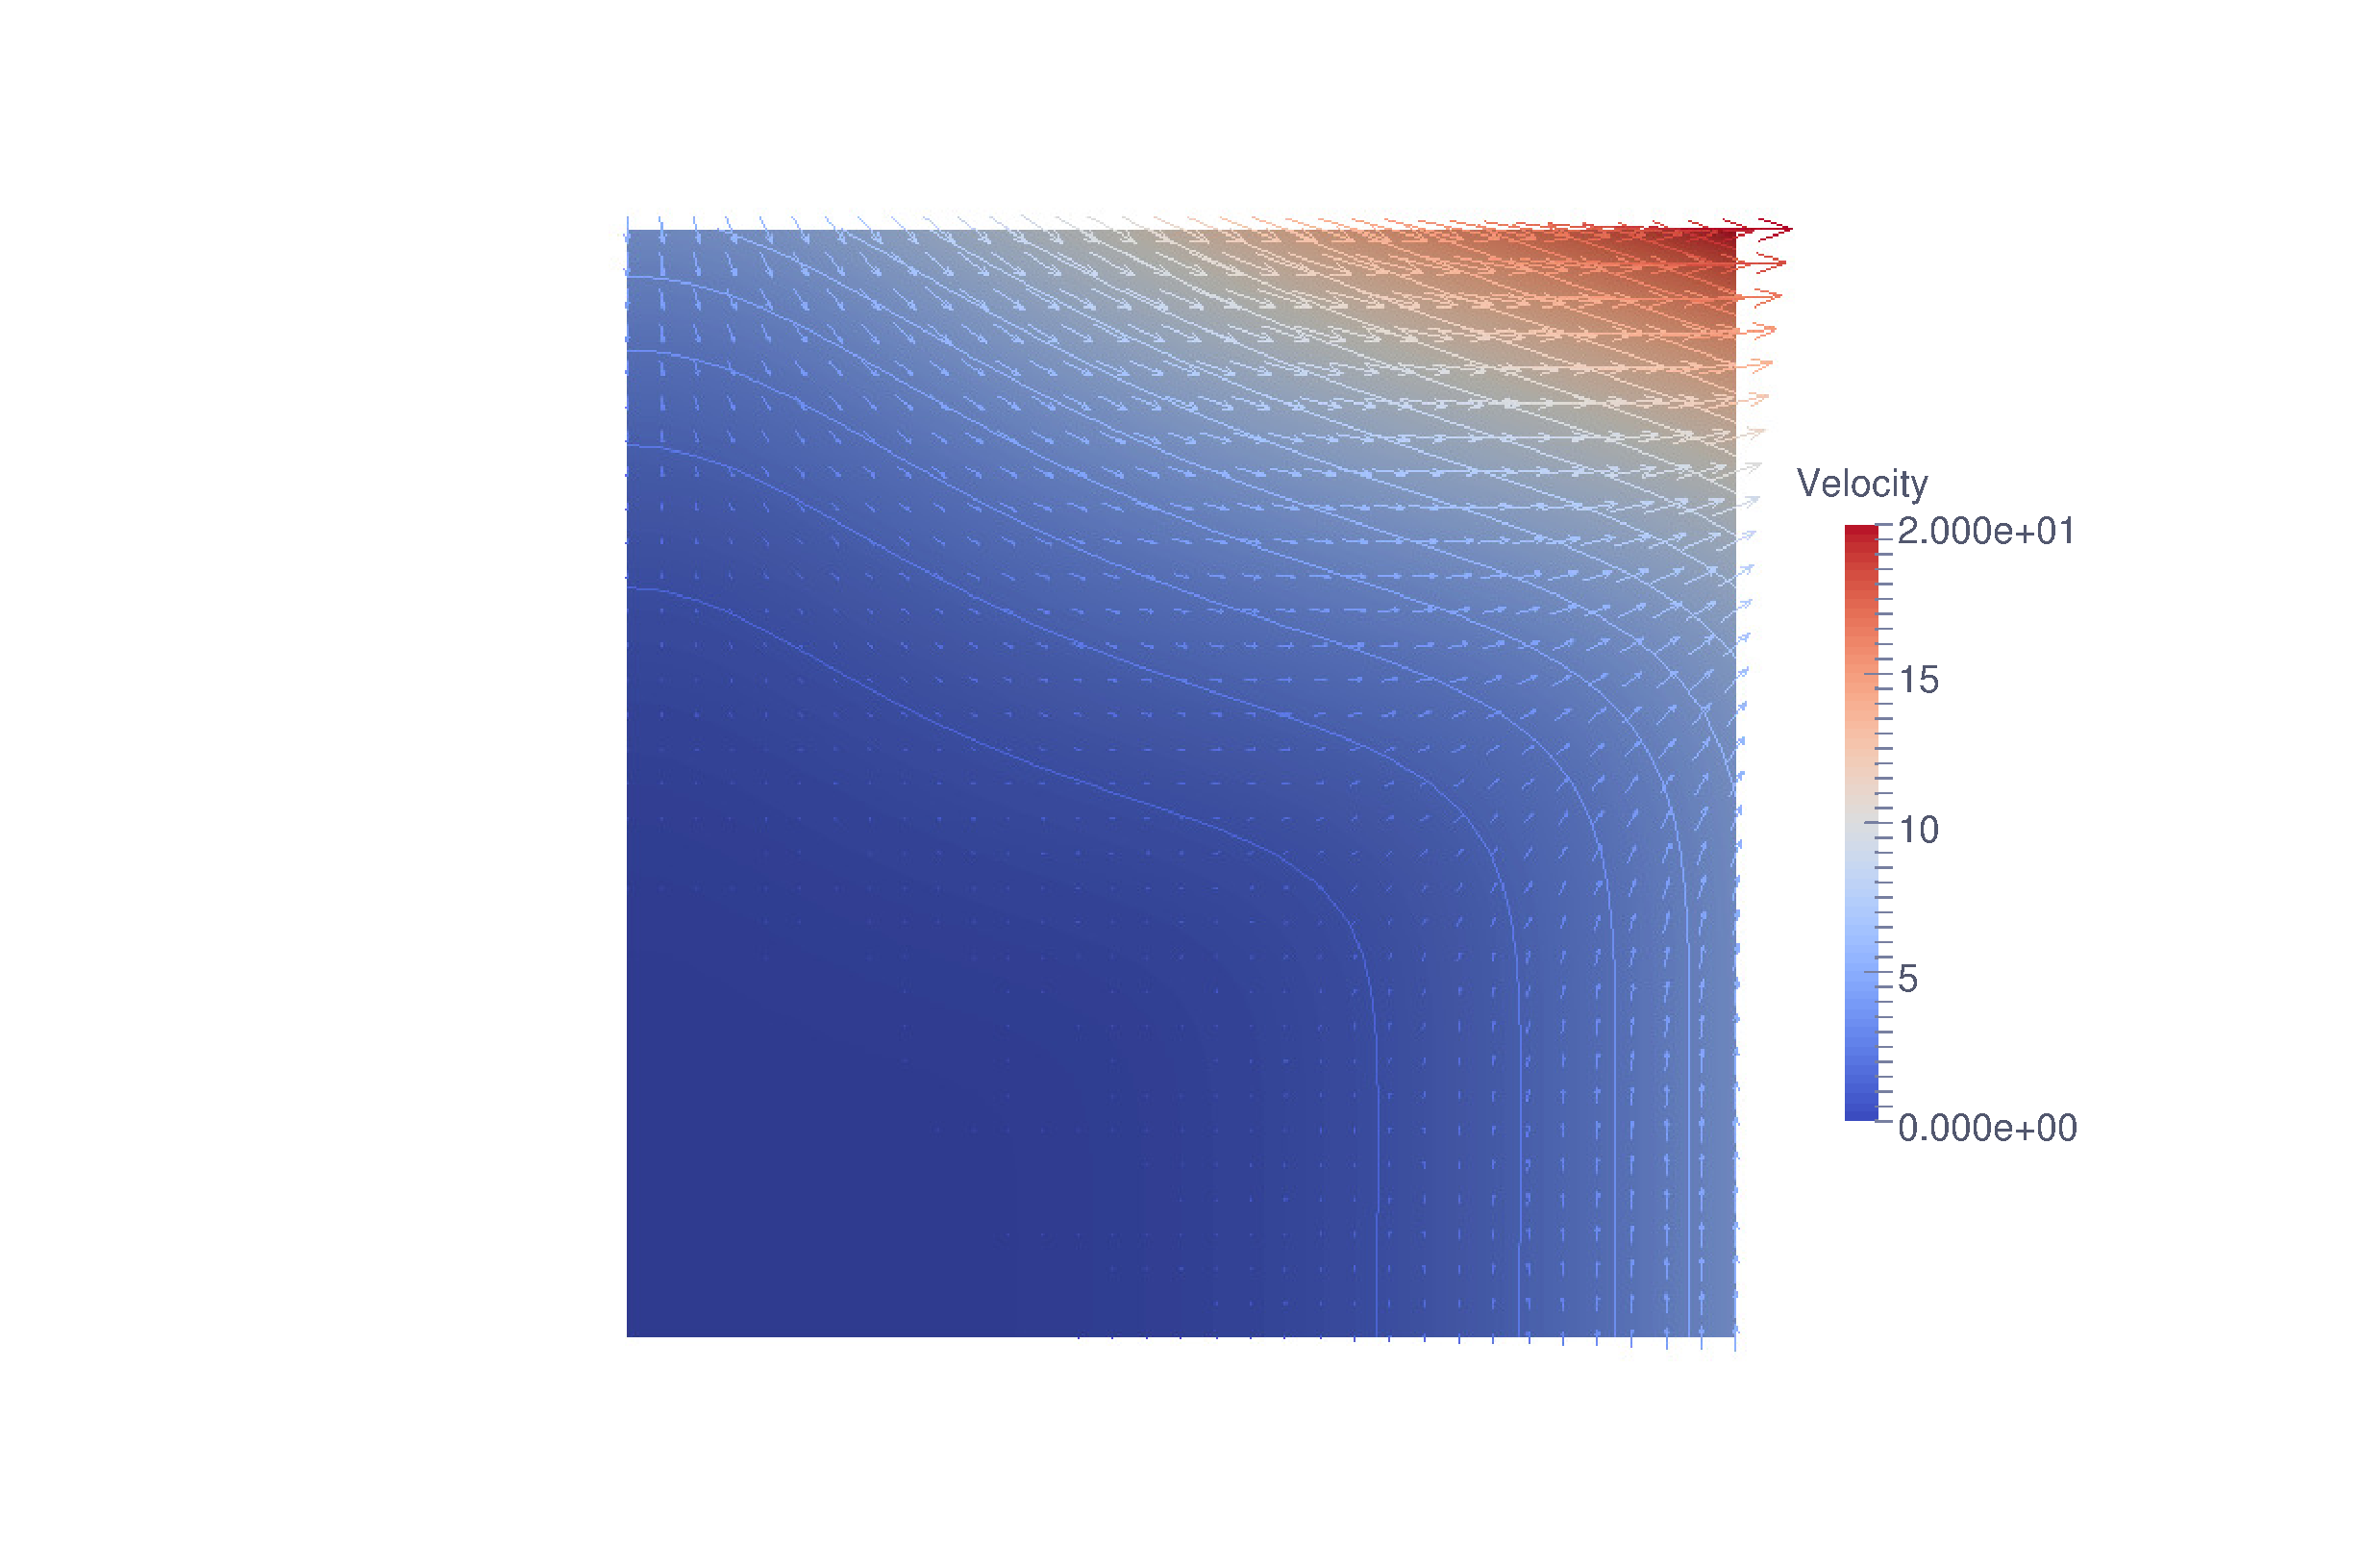
\includegraphics[trim=10cm 3.5cm 5cm 3cm, clip=true, width=0.5\textwidth]{Figures/colliding_flow.pdf}
	\vspace*{-0.2cm}
	\caption{Velocity field}
  \end{figure}
\end{frame}
%----------------------------------------------------------------------------------------
\begin{frame}
 \frametitle{Colliding flow}
 \textbf{Acumulated solver iterations:} (using $ P_U(\overset{\tilde{}}{A}) $)
  \vspace*{-0.3cm}
 \begin{figure}
     \centering	
     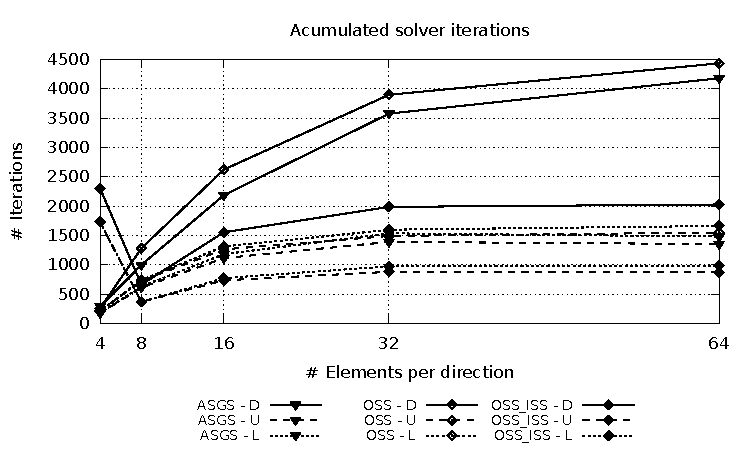
\includegraphics[width=0.8\textwidth]{Figures/colliding_iter.pdf}
   \end{figure}
 \begin{overlayarea}{\textwidth}{1.5cm}
 \only<2->{
 \vspace*{-0.6cm}
 \begin{itemize}
  	\item \alert<2>{$ P_U(\overset{\tilde{}}{K}_\tau) $ and $ P_L(\overset{\tilde{}}{K}_\tau) $ scalable block-preconditioners} for all methods.
  	\only<3->{\item \alert<3>{Less solver iterations for the OSS-ISS method} with the same velocity DOFs.}
  \end{itemize}}
  \end{overlayarea}
\end{frame}
%----------------------------------------------------------------------------------------
\begin{frame}
 \frametitle{Colliding flow}
 \textbf{Accuracy:} \only<1-2>{Velocity error}\only<3-4>{Pressure error}
   \vspace*{-0.3cm}
 \only<1-3>{
 \begin{figure}
     \centering	
     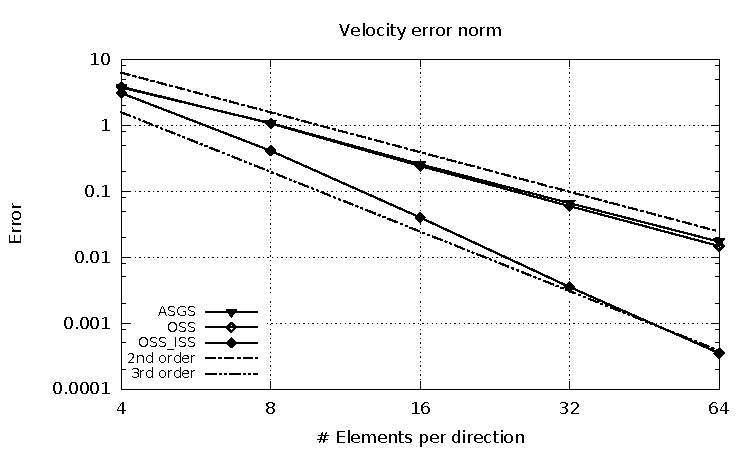
\includegraphics[width=0.8\textwidth]{Figures/colliding_erru.pdf}
   \end{figure}}
\only<4->{
\begin{figure}
    \centering	
    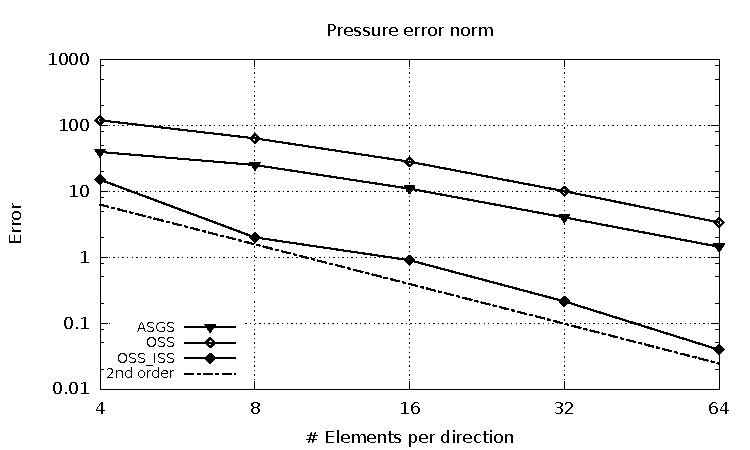
\includegraphics[width=0.8\textwidth]{Figures/colliding_errp.pdf}
  \end{figure}}
 \begin{overlayarea}{\textwidth}{1.5cm}
  \vspace*{-0.5cm}
 \only<2-3>{
 \begin{itemize}
  	\item \alert<2>{2nd order} convergence rate for ASGS and OSS methods.
  	\only<3->{\item \alert<3>{3rd order} convergence rate for OSS-ISS method.}
  \end{itemize}}
   \only<5->{
   \begin{itemize}
    	\item \alert<5>{2nd order} convergence rate for all methods.
    	\only<6->{\item \alert<6>{Best accuracy for OSS-ISS method}.}
    \end{itemize}}
  \end{overlayarea}
\end{frame}
%----------------------------------------------------------------------------------------
\begin{frame}
 \frametitle{Colliding flow}
 \textbf{Efficiency:} \only<1-2>{Velocity}\only<3>{Pressure}
   \vspace*{-0.3cm}
 \only<1-2>{
 \begin{figure}
     \centering	
     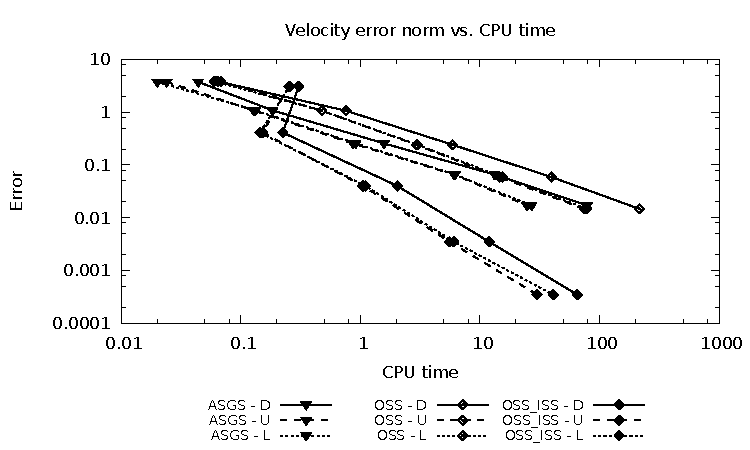
\includegraphics[width=0.8\textwidth]{Figures/colliding_errtu.pdf}
   \end{figure}}
\only<3->{
\begin{figure}
    \centering	
    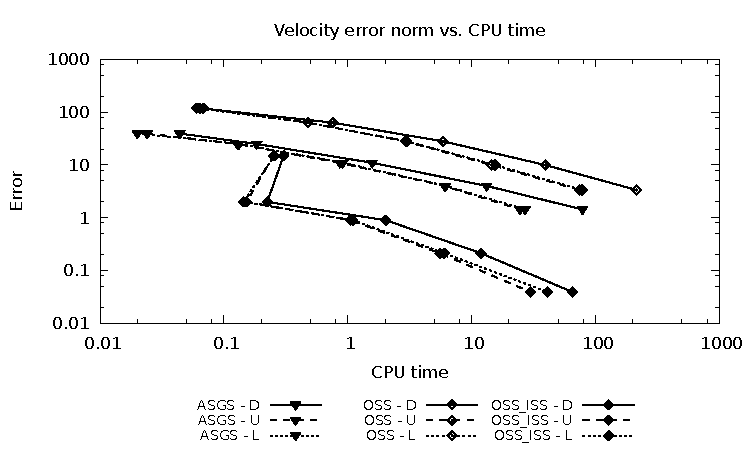
\includegraphics[width=0.8\textwidth]{Figures/colliding_errtp.pdf}
  \end{figure}}
 \begin{overlayarea}{\textwidth}{1.5cm}
  \vspace*{-0.5cm}
 \only<2>{
 \begin{itemize}
  	\item \alert<2>{OSS-ISS the most efficient method}.
  \end{itemize}}
   \only<3->{
   \begin{itemize}
    	\item \alert<3>{Also for pressures.}
    \end{itemize}}
  \end{overlayarea}
\end{frame}